% Created by tikzDevice version 0.12.3.1 on 2022-05-01 19:43:58
% !TEX encoding = UTF-8 Unicode
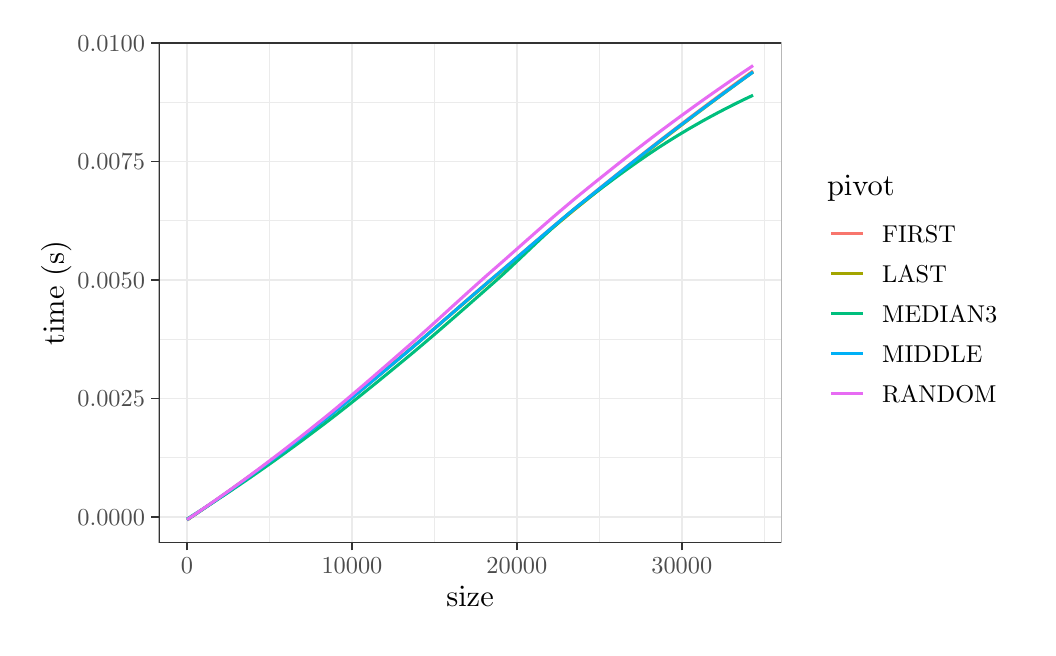
\begin{tikzpicture}[x=1pt,y=1pt]
\definecolor{fillColor}{RGB}{255,255,255}
\path[use as bounding box,fill=fillColor,fill opacity=0.00] (0,0) rectangle (361.35,216.81);
\begin{scope}
\path[clip] (  0.00,  0.00) rectangle (361.35,216.81);
\definecolor{drawColor}{RGB}{255,255,255}
\definecolor{fillColor}{RGB}{255,255,255}

\path[draw=drawColor,line width= 0.6pt,line join=round,line cap=round,fill=fillColor] (  0.00,  0.00) rectangle (361.35,216.81);
\end{scope}
\begin{scope}
\path[clip] ( 47.35, 30.69) rectangle (272.35,211.31);
\definecolor{fillColor}{RGB}{255,255,255}

\path[fill=fillColor] ( 47.35, 30.69) rectangle (272.35,211.31);
\definecolor{drawColor}{gray}{0.92}

\path[draw=drawColor,line width= 0.3pt,line join=round] ( 47.35, 61.46) --
	(272.35, 61.46);

\path[draw=drawColor,line width= 0.3pt,line join=round] ( 47.35,104.25) --
	(272.35,104.25);

\path[draw=drawColor,line width= 0.3pt,line join=round] ( 47.35,147.04) --
	(272.35,147.04);

\path[draw=drawColor,line width= 0.3pt,line join=round] ( 47.35,189.82) --
	(272.35,189.82);

\path[draw=drawColor,line width= 0.3pt,line join=round] ( 87.38, 30.69) --
	( 87.38,211.31);

\path[draw=drawColor,line width= 0.3pt,line join=round] (146.97, 30.69) --
	(146.97,211.31);

\path[draw=drawColor,line width= 0.3pt,line join=round] (206.57, 30.69) --
	(206.57,211.31);

\path[draw=drawColor,line width= 0.3pt,line join=round] (266.16, 30.69) --
	(266.16,211.31);

\path[draw=drawColor,line width= 0.6pt,line join=round] ( 47.35, 40.07) --
	(272.35, 40.07);

\path[draw=drawColor,line width= 0.6pt,line join=round] ( 47.35, 82.85) --
	(272.35, 82.85);

\path[draw=drawColor,line width= 0.6pt,line join=round] ( 47.35,125.64) --
	(272.35,125.64);

\path[draw=drawColor,line width= 0.6pt,line join=round] ( 47.35,168.43) --
	(272.35,168.43);

\path[draw=drawColor,line width= 0.6pt,line join=round] ( 47.35,211.22) --
	(272.35,211.22);

\path[draw=drawColor,line width= 0.6pt,line join=round] ( 57.58, 30.69) --
	( 57.58,211.31);

\path[draw=drawColor,line width= 0.6pt,line join=round] (117.18, 30.69) --
	(117.18,211.31);

\path[draw=drawColor,line width= 0.6pt,line join=round] (176.77, 30.69) --
	(176.77,211.31);

\path[draw=drawColor,line width= 0.6pt,line join=round] (236.37, 30.69) --
	(236.37,211.31);
\definecolor{drawColor}{RGB}{248,118,109}

\path[draw=drawColor,line width= 1.1pt,line join=round] ( 57.58, 38.99) --
	( 60.17, 40.72) --
	( 62.76, 42.46) --
	( 65.35, 44.23) --
	( 67.94, 46.01) --
	( 70.53, 47.81) --
	( 73.12, 49.63) --
	( 75.70, 51.46) --
	( 78.29, 53.31) --
	( 80.88, 55.18) --
	( 83.47, 57.06) --
	( 86.06, 58.96) --
	( 88.65, 60.88) --
	( 91.24, 62.82) --
	( 93.83, 64.77) --
	( 96.42, 66.74) --
	( 99.01, 68.72) --
	(101.60, 70.71) --
	(104.18, 72.72) --
	(106.77, 74.74) --
	(109.36, 76.79) --
	(111.95, 78.86) --
	(114.54, 80.95) --
	(117.13, 83.06) --
	(119.72, 85.18) --
	(122.31, 87.32) --
	(124.90, 89.47) --
	(127.49, 91.63) --
	(130.08, 93.79) --
	(132.67, 95.96) --
	(135.25, 98.14) --
	(137.84,100.31) --
	(140.43,102.51) --
	(143.02,104.72) --
	(145.61,106.96) --
	(148.20,109.20) --
	(150.79,111.46) --
	(153.38,113.71) --
	(155.97,115.97) --
	(158.56,118.22) --
	(161.15,120.46) --
	(163.74,122.68) --
	(166.32,124.89) --
	(168.91,127.08) --
	(171.50,129.28) --
	(174.09,131.48) --
	(176.68,133.70) --
	(179.27,135.91) --
	(181.86,138.13) --
	(184.45,140.34) --
	(187.04,142.55) --
	(189.63,144.74) --
	(192.22,146.92) --
	(194.81,149.08) --
	(197.39,151.22) --
	(199.98,153.34) --
	(202.57,155.44) --
	(205.16,157.53) --
	(207.75,159.62) --
	(210.34,161.70) --
	(212.93,163.78) --
	(215.52,165.84) --
	(218.11,167.90) --
	(220.70,169.94) --
	(223.29,171.98) --
	(225.88,174.00) --
	(228.46,176.01) --
	(231.05,178.01) --
	(233.64,180.00) --
	(236.23,181.97) --
	(238.82,183.94) --
	(241.41,185.89) --
	(244.00,187.83) --
	(246.59,189.77) --
	(249.18,191.69) --
	(251.77,193.60) --
	(254.36,195.51) --
	(256.94,197.40) --
	(259.53,199.28) --
	(262.12,201.16);
\definecolor{drawColor}{RGB}{163,165,0}

\path[draw=drawColor,line width= 1.1pt,line join=round] ( 57.58, 38.90) --
	( 60.17, 40.65) --
	( 62.76, 42.41) --
	( 65.35, 44.19) --
	( 67.94, 45.99) --
	( 70.53, 47.80) --
	( 73.12, 49.63) --
	( 75.70, 51.48) --
	( 78.29, 53.34) --
	( 80.88, 55.22) --
	( 83.47, 57.11) --
	( 86.06, 59.02) --
	( 88.65, 60.94) --
	( 91.24, 62.89) --
	( 93.83, 64.84) --
	( 96.42, 66.81) --
	( 99.01, 68.80) --
	(101.60, 70.79) --
	(104.18, 72.80) --
	(106.77, 74.82) --
	(109.36, 76.87) --
	(111.95, 78.93) --
	(114.54, 81.02) --
	(117.13, 83.12) --
	(119.72, 85.24) --
	(122.31, 87.37) --
	(124.90, 89.51) --
	(127.49, 91.66) --
	(130.08, 93.81) --
	(132.67, 95.97) --
	(135.25, 98.13) --
	(137.84,100.29) --
	(140.43,102.47) --
	(143.02,104.67) --
	(145.61,106.88) --
	(148.20,109.10) --
	(150.79,111.33) --
	(153.38,113.56) --
	(155.97,115.79) --
	(158.56,118.02) --
	(161.15,120.24) --
	(163.74,122.44) --
	(166.32,124.64) --
	(168.91,126.81) --
	(171.50,129.00) --
	(174.09,131.19) --
	(176.68,133.40) --
	(179.27,135.61) --
	(181.86,137.82) --
	(184.45,140.02) --
	(187.04,142.22) --
	(189.63,144.41) --
	(192.22,146.58) --
	(194.81,148.73) --
	(197.39,150.87) --
	(199.98,152.97) --
	(202.57,155.07) --
	(205.16,157.16) --
	(207.75,159.25) --
	(210.34,161.32) --
	(212.93,163.39) --
	(215.52,165.46) --
	(218.11,167.51) --
	(220.70,169.55) --
	(223.29,171.58) --
	(225.88,173.61) --
	(228.46,175.62) --
	(231.05,177.61) --
	(233.64,179.60) --
	(236.23,181.58) --
	(238.82,183.54) --
	(241.41,185.50) --
	(244.00,187.44) --
	(246.59,189.38) --
	(249.18,191.30) --
	(251.77,193.21) --
	(254.36,195.12) --
	(256.94,197.02) --
	(259.53,198.90) --
	(262.12,200.78);
\definecolor{drawColor}{RGB}{0,191,125}

\path[draw=drawColor,line width= 1.1pt,line join=round] ( 57.58, 39.26) --
	( 60.17, 40.89) --
	( 62.76, 42.53) --
	( 65.35, 44.19) --
	( 67.94, 45.87) --
	( 70.53, 47.57) --
	( 73.12, 49.29) --
	( 75.70, 51.04) --
	( 78.29, 52.79) --
	( 80.88, 54.57) --
	( 83.47, 56.36) --
	( 86.06, 58.18) --
	( 88.65, 60.01) --
	( 91.24, 61.87) --
	( 93.83, 63.74) --
	( 96.42, 65.63) --
	( 99.01, 67.53) --
	(101.60, 69.46) --
	(104.18, 71.39) --
	(106.77, 73.34) --
	(109.36, 75.32) --
	(111.95, 77.32) --
	(114.54, 79.35) --
	(117.13, 81.39) --
	(119.72, 83.45) --
	(122.31, 85.53) --
	(124.90, 87.62) --
	(127.49, 89.72) --
	(130.08, 91.84) --
	(132.67, 93.96) --
	(135.25, 96.09) --
	(137.84, 98.23) --
	(140.43,100.39) --
	(143.02,102.58) --
	(145.61,104.78) --
	(148.20,107.00) --
	(150.79,109.24) --
	(153.38,111.49) --
	(155.97,113.75) --
	(158.56,116.01) --
	(161.15,118.29) --
	(163.74,120.56) --
	(166.32,122.83) --
	(168.91,125.11) --
	(171.50,127.44) --
	(174.09,129.83) --
	(176.68,132.26) --
	(179.27,134.72) --
	(181.86,137.18) --
	(184.45,139.63) --
	(187.04,142.06) --
	(189.63,144.44) --
	(192.22,146.76) --
	(194.81,149.01) --
	(197.39,151.16) --
	(199.98,153.20) --
	(202.57,155.20) --
	(205.16,157.18) --
	(207.75,159.14) --
	(210.34,161.08) --
	(212.93,162.99) --
	(215.52,164.88) --
	(218.11,166.73) --
	(220.70,168.55) --
	(223.29,170.34) --
	(225.88,172.09) --
	(228.46,173.79) --
	(231.05,175.45) --
	(233.64,177.07) --
	(236.23,178.65) --
	(238.82,180.19) --
	(241.41,181.68) --
	(244.00,183.15) --
	(246.59,184.57) --
	(249.18,185.96) --
	(251.77,187.31) --
	(254.36,188.63) --
	(256.94,189.92) --
	(259.53,191.17) --
	(262.12,192.39);
\definecolor{drawColor}{RGB}{0,176,246}

\path[draw=drawColor,line width= 1.1pt,line join=round] ( 57.58, 38.98) --
	( 60.17, 40.71) --
	( 62.76, 42.46) --
	( 65.35, 44.23) --
	( 67.94, 46.01) --
	( 70.53, 47.82) --
	( 73.12, 49.64) --
	( 75.70, 51.47) --
	( 78.29, 53.32) --
	( 80.88, 55.19) --
	( 83.47, 57.07) --
	( 86.06, 58.97) --
	( 88.65, 60.89) --
	( 91.24, 62.83) --
	( 93.83, 64.78) --
	( 96.42, 66.74) --
	( 99.01, 68.72) --
	(101.60, 70.71) --
	(104.18, 72.72) --
	(106.77, 74.74) --
	(109.36, 76.78) --
	(111.95, 78.84) --
	(114.54, 80.93) --
	(117.13, 83.03) --
	(119.72, 85.15) --
	(122.31, 87.28) --
	(124.90, 89.42) --
	(127.49, 91.58) --
	(130.08, 93.74) --
	(132.67, 95.90) --
	(135.25, 98.07) --
	(137.84,100.24) --
	(140.43,102.43) --
	(143.02,104.65) --
	(145.61,106.88) --
	(148.20,109.12) --
	(150.79,111.38) --
	(153.38,113.63) --
	(155.97,115.89) --
	(158.56,118.14) --
	(161.15,120.38) --
	(163.74,122.61) --
	(166.32,124.82) --
	(168.91,127.01) --
	(171.50,129.21) --
	(174.09,131.42) --
	(176.68,133.63) --
	(179.27,135.85) --
	(181.86,138.07) --
	(184.45,140.29) --
	(187.04,142.49) --
	(189.63,144.69) --
	(192.22,146.87) --
	(194.81,149.03) --
	(197.39,151.16) --
	(199.98,153.27) --
	(202.57,155.36) --
	(205.16,157.45) --
	(207.75,159.53) --
	(210.34,161.61) --
	(212.93,163.67) --
	(215.52,165.73) --
	(218.11,167.78) --
	(220.70,169.81) --
	(223.29,171.84) --
	(225.88,173.85) --
	(228.46,175.85) --
	(231.05,177.84) --
	(233.64,179.81) --
	(236.23,181.77) --
	(238.82,183.72) --
	(241.41,185.66) --
	(244.00,187.59) --
	(246.59,189.50) --
	(249.18,191.41) --
	(251.77,193.31) --
	(254.36,195.19) --
	(256.94,197.06) --
	(259.53,198.93) --
	(262.12,200.78);
\definecolor{drawColor}{RGB}{231,107,243}

\path[draw=drawColor,line width= 1.1pt,line join=round] ( 57.58, 39.04) --
	( 60.17, 40.78) --
	( 62.76, 42.54) --
	( 65.35, 44.32) --
	( 67.94, 46.12) --
	( 70.53, 47.94) --
	( 73.12, 49.78) --
	( 75.70, 51.64) --
	( 78.29, 53.52) --
	( 80.88, 55.42) --
	( 83.47, 57.34) --
	( 86.06, 59.28) --
	( 88.65, 61.24) --
	( 91.24, 63.22) --
	( 93.83, 65.21) --
	( 96.42, 67.23) --
	( 99.01, 69.26) --
	(101.60, 71.31) --
	(104.18, 73.38) --
	(106.77, 75.46) --
	(109.36, 77.57) --
	(111.95, 79.71) --
	(114.54, 81.88) --
	(117.13, 84.07) --
	(119.72, 86.27) --
	(122.31, 88.50) --
	(124.90, 90.73) --
	(127.49, 92.98) --
	(130.08, 95.23) --
	(132.67, 97.49) --
	(135.25, 99.75) --
	(137.84,102.01) --
	(140.43,104.29) --
	(143.02,106.61) --
	(145.61,108.94) --
	(148.20,111.28) --
	(150.79,113.64) --
	(153.38,116.00) --
	(155.97,118.35) --
	(158.56,120.70) --
	(161.15,123.03) --
	(163.74,125.35) --
	(166.32,127.64) --
	(168.91,129.90) --
	(171.50,132.17) --
	(174.09,134.46) --
	(176.68,136.75) --
	(179.27,139.04) --
	(181.86,141.33) --
	(184.45,143.62) --
	(187.04,145.89) --
	(189.63,148.14) --
	(192.22,150.37) --
	(194.81,152.56) --
	(197.39,154.73) --
	(199.98,156.85) --
	(202.57,158.96) --
	(205.16,161.05) --
	(207.75,163.13) --
	(210.34,165.20) --
	(212.93,167.26) --
	(215.52,169.30) --
	(218.11,171.33) --
	(220.70,173.34) --
	(223.29,175.33) --
	(225.88,177.31) --
	(228.46,179.26) --
	(231.05,181.20) --
	(233.64,183.12) --
	(236.23,185.02) --
	(238.82,186.90) --
	(241.41,188.77) --
	(244.00,190.62) --
	(246.59,192.45) --
	(249.18,194.26) --
	(251.77,196.06) --
	(254.36,197.85) --
	(256.94,199.61) --
	(259.53,201.36) --
	(262.12,203.10);
\definecolor{drawColor}{gray}{0.20}

\path[draw=drawColor,line width= 0.6pt,line join=round,line cap=round] ( 47.35, 30.69) rectangle (272.35,211.31);
\end{scope}
\begin{scope}
\path[clip] (  0.00,  0.00) rectangle (361.35,216.81);
\definecolor{drawColor}{gray}{0.30}

\node[text=drawColor,anchor=base east,inner sep=0pt, outer sep=0pt, scale=  0.88] at ( 42.40, 37.04) {0.0000};

\node[text=drawColor,anchor=base east,inner sep=0pt, outer sep=0pt, scale=  0.88] at ( 42.40, 79.82) {0.0025};

\node[text=drawColor,anchor=base east,inner sep=0pt, outer sep=0pt, scale=  0.88] at ( 42.40,122.61) {0.0050};

\node[text=drawColor,anchor=base east,inner sep=0pt, outer sep=0pt, scale=  0.88] at ( 42.40,165.40) {0.0075};

\node[text=drawColor,anchor=base east,inner sep=0pt, outer sep=0pt, scale=  0.88] at ( 42.40,208.19) {0.0100};
\end{scope}
\begin{scope}
\path[clip] (  0.00,  0.00) rectangle (361.35,216.81);
\definecolor{drawColor}{gray}{0.20}

\path[draw=drawColor,line width= 0.6pt,line join=round] ( 44.60, 40.07) --
	( 47.35, 40.07);

\path[draw=drawColor,line width= 0.6pt,line join=round] ( 44.60, 82.85) --
	( 47.35, 82.85);

\path[draw=drawColor,line width= 0.6pt,line join=round] ( 44.60,125.64) --
	( 47.35,125.64);

\path[draw=drawColor,line width= 0.6pt,line join=round] ( 44.60,168.43) --
	( 47.35,168.43);

\path[draw=drawColor,line width= 0.6pt,line join=round] ( 44.60,211.22) --
	( 47.35,211.22);
\end{scope}
\begin{scope}
\path[clip] (  0.00,  0.00) rectangle (361.35,216.81);
\definecolor{drawColor}{gray}{0.20}

\path[draw=drawColor,line width= 0.6pt,line join=round] ( 57.58, 27.94) --
	( 57.58, 30.69);

\path[draw=drawColor,line width= 0.6pt,line join=round] (117.18, 27.94) --
	(117.18, 30.69);

\path[draw=drawColor,line width= 0.6pt,line join=round] (176.77, 27.94) --
	(176.77, 30.69);

\path[draw=drawColor,line width= 0.6pt,line join=round] (236.37, 27.94) --
	(236.37, 30.69);
\end{scope}
\begin{scope}
\path[clip] (  0.00,  0.00) rectangle (361.35,216.81);
\definecolor{drawColor}{gray}{0.30}

\node[text=drawColor,anchor=base,inner sep=0pt, outer sep=0pt, scale=  0.88] at ( 57.58, 19.68) {0};

\node[text=drawColor,anchor=base,inner sep=0pt, outer sep=0pt, scale=  0.88] at (117.18, 19.68) {10000};

\node[text=drawColor,anchor=base,inner sep=0pt, outer sep=0pt, scale=  0.88] at (176.77, 19.68) {20000};

\node[text=drawColor,anchor=base,inner sep=0pt, outer sep=0pt, scale=  0.88] at (236.37, 19.68) {30000};
\end{scope}
\begin{scope}
\path[clip] (  0.00,  0.00) rectangle (361.35,216.81);
\definecolor{drawColor}{RGB}{0,0,0}

\node[text=drawColor,anchor=base,inner sep=0pt, outer sep=0pt, scale=  1.10] at (159.85,  7.64) {size};
\end{scope}
\begin{scope}
\path[clip] (  0.00,  0.00) rectangle (361.35,216.81);
\definecolor{drawColor}{RGB}{0,0,0}

\node[text=drawColor,rotate= 90.00,anchor=base,inner sep=0pt, outer sep=0pt, scale=  1.10] at ( 13.08,121.00) {time (s)};
\end{scope}
\begin{scope}
\path[clip] (  0.00,  0.00) rectangle (361.35,216.81);
\definecolor{fillColor}{RGB}{255,255,255}

\path[fill=fillColor] (283.35, 71.76) rectangle (355.85,170.24);
\end{scope}
\begin{scope}
\path[clip] (  0.00,  0.00) rectangle (361.35,216.81);
\definecolor{drawColor}{RGB}{0,0,0}

\node[text=drawColor,anchor=base west,inner sep=0pt, outer sep=0pt, scale=  1.10] at (288.85,156.09) {pivot};
\end{scope}
\begin{scope}
\path[clip] (  0.00,  0.00) rectangle (361.35,216.81);
\definecolor{fillColor}{RGB}{255,255,255}

\path[fill=fillColor] (288.85,135.07) rectangle (303.30,149.53);
\end{scope}
\begin{scope}
\path[clip] (  0.00,  0.00) rectangle (361.35,216.81);
\definecolor{drawColor}{RGB}{248,118,109}

\path[draw=drawColor,line width= 1.1pt,line join=round] (290.30,142.30) -- (301.86,142.30);
\end{scope}
\begin{scope}
\path[clip] (  0.00,  0.00) rectangle (361.35,216.81);
\definecolor{fillColor}{RGB}{255,255,255}

\path[fill=fillColor] (288.85,120.62) rectangle (303.30,135.07);
\end{scope}
\begin{scope}
\path[clip] (  0.00,  0.00) rectangle (361.35,216.81);
\definecolor{drawColor}{RGB}{163,165,0}

\path[draw=drawColor,line width= 1.1pt,line join=round] (290.30,127.84) -- (301.86,127.84);
\end{scope}
\begin{scope}
\path[clip] (  0.00,  0.00) rectangle (361.35,216.81);
\definecolor{fillColor}{RGB}{255,255,255}

\path[fill=fillColor] (288.85,106.16) rectangle (303.30,120.62);
\end{scope}
\begin{scope}
\path[clip] (  0.00,  0.00) rectangle (361.35,216.81);
\definecolor{drawColor}{RGB}{0,191,125}

\path[draw=drawColor,line width= 1.1pt,line join=round] (290.30,113.39) -- (301.86,113.39);
\end{scope}
\begin{scope}
\path[clip] (  0.00,  0.00) rectangle (361.35,216.81);
\definecolor{fillColor}{RGB}{255,255,255}

\path[fill=fillColor] (288.85, 91.71) rectangle (303.30,106.16);
\end{scope}
\begin{scope}
\path[clip] (  0.00,  0.00) rectangle (361.35,216.81);
\definecolor{drawColor}{RGB}{0,176,246}

\path[draw=drawColor,line width= 1.1pt,line join=round] (290.30, 98.94) -- (301.86, 98.94);
\end{scope}
\begin{scope}
\path[clip] (  0.00,  0.00) rectangle (361.35,216.81);
\definecolor{fillColor}{RGB}{255,255,255}

\path[fill=fillColor] (288.85, 77.26) rectangle (303.30, 91.71);
\end{scope}
\begin{scope}
\path[clip] (  0.00,  0.00) rectangle (361.35,216.81);
\definecolor{drawColor}{RGB}{231,107,243}

\path[draw=drawColor,line width= 1.1pt,line join=round] (290.30, 84.48) -- (301.86, 84.48);
\end{scope}
\begin{scope}
\path[clip] (  0.00,  0.00) rectangle (361.35,216.81);
\definecolor{drawColor}{RGB}{0,0,0}

\node[text=drawColor,anchor=base west,inner sep=0pt, outer sep=0pt, scale=  0.88] at (308.80,139.27) {FIRST};
\end{scope}
\begin{scope}
\path[clip] (  0.00,  0.00) rectangle (361.35,216.81);
\definecolor{drawColor}{RGB}{0,0,0}

\node[text=drawColor,anchor=base west,inner sep=0pt, outer sep=0pt, scale=  0.88] at (308.80,124.81) {LAST};
\end{scope}
\begin{scope}
\path[clip] (  0.00,  0.00) rectangle (361.35,216.81);
\definecolor{drawColor}{RGB}{0,0,0}

\node[text=drawColor,anchor=base west,inner sep=0pt, outer sep=0pt, scale=  0.88] at (308.80,110.36) {MEDIAN3};
\end{scope}
\begin{scope}
\path[clip] (  0.00,  0.00) rectangle (361.35,216.81);
\definecolor{drawColor}{RGB}{0,0,0}

\node[text=drawColor,anchor=base west,inner sep=0pt, outer sep=0pt, scale=  0.88] at (308.80, 95.91) {MIDDLE};
\end{scope}
\begin{scope}
\path[clip] (  0.00,  0.00) rectangle (361.35,216.81);
\definecolor{drawColor}{RGB}{0,0,0}

\node[text=drawColor,anchor=base west,inner sep=0pt, outer sep=0pt, scale=  0.88] at (308.80, 81.45) {RANDOM};
\end{scope}
\end{tikzpicture}
